\documentclass[reprint,floatfix,amsmath,amssymb,aps,pra]{revtex4-1}

\usepackage{dragly-revtex}

\usepackage{}

\begin{document}

\title{FYS4460 Project 1}
\author{Svenn-Arne Dragly}

\begin{abstract}
In this project we study a monatomic gas consisting of Argon atoms using molecular dynamics.
\end{abstract}

\maketitle

\section{Introduction}

\section{Theory}

\subsection{Integration}

We assume that our particles adhere to Newtonian motion based on the interatomic forces and use the velocity-Verlet method to integrate motion in our system.

\subsection{Interatomic force}

The interatomic force is based on a chosen Lennard-Jones potential.
\begin{equation}
    V_{LJ} = 4 \varepsilon \left[ \left( \frac {\sigma} {r} \right)^{12} - \left( \frac {\sigma} {r} \right)^6 \right]
\end{equation}
where $r$ is the distance between two atoms, $\sigma$ is chosen to be $\sigma = 3.405 \unit{\AA}$ and $\varepsilon = 1.0318 \cdot 10^{−2} \unit{eV}$.

Taking the gradient of the potential gives us the force as
\begin{equation}
 \vec F = \frac{24 \varepsilon}{r^{2}} \left[ \left( 2 \frac {\sigma} {r} \right)^{12} - \left( \frac {\sigma} {r} \right)^6 \right] \vec r
\end{equation}

\section{Implementation}

\subsection{Initial velocities and temperature}

To mimic a given temperature upon starting the system, we select speeds from a Boltzmann distribution, meaning that the x-, y- and z-components of the velocity have zero mean and standard deviation $\sqrt{k_{B}T / m}$.

\subsection{Periodic boundary conditions}

Our system is limited in size, but to mimic a larger system, we use periodic boundary conditions. 

\subsection{Neighbor cells}

To make the calculations go faster, we decide on a cutoff distance for the force. Outside this cutoff distance, we assume that the interatomic force is zero. Inside, it is still defined by the Lennard-Jones potential. In this project, we set the cutoff distance to be $r_{\text{cut}} = 3 \sigma$.

To make use of this, we implement neighbor cells\footnote{Neighbor cells are generally easier to combine with parallel code. Another approach is to use Verlet lists.} as a division of our space into regions at least as large as $r_{\text{cut}}$ in all directions.

\section{Results}

\subsection{Boltzmann distribution of velocities}

\begin{figure*}
    \centering
    \subfigure[]{
        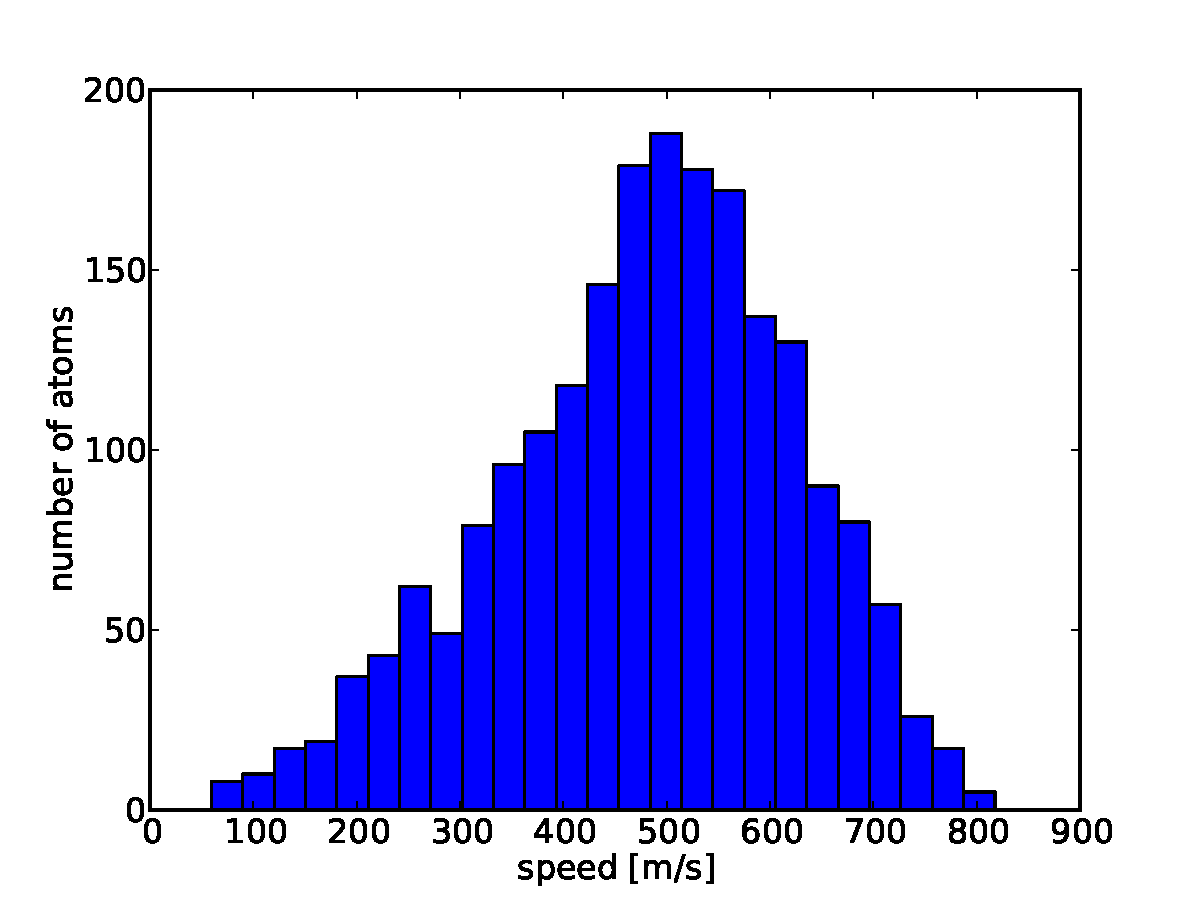
\includegraphics[width=0.48\textwidth]{./analysis/1i-boltzmann/runs/2013-02-26_180246/data000000-norm.pdf}
    } \label{fig:velocity-magnitudes-first}
    \subfigure[]{
	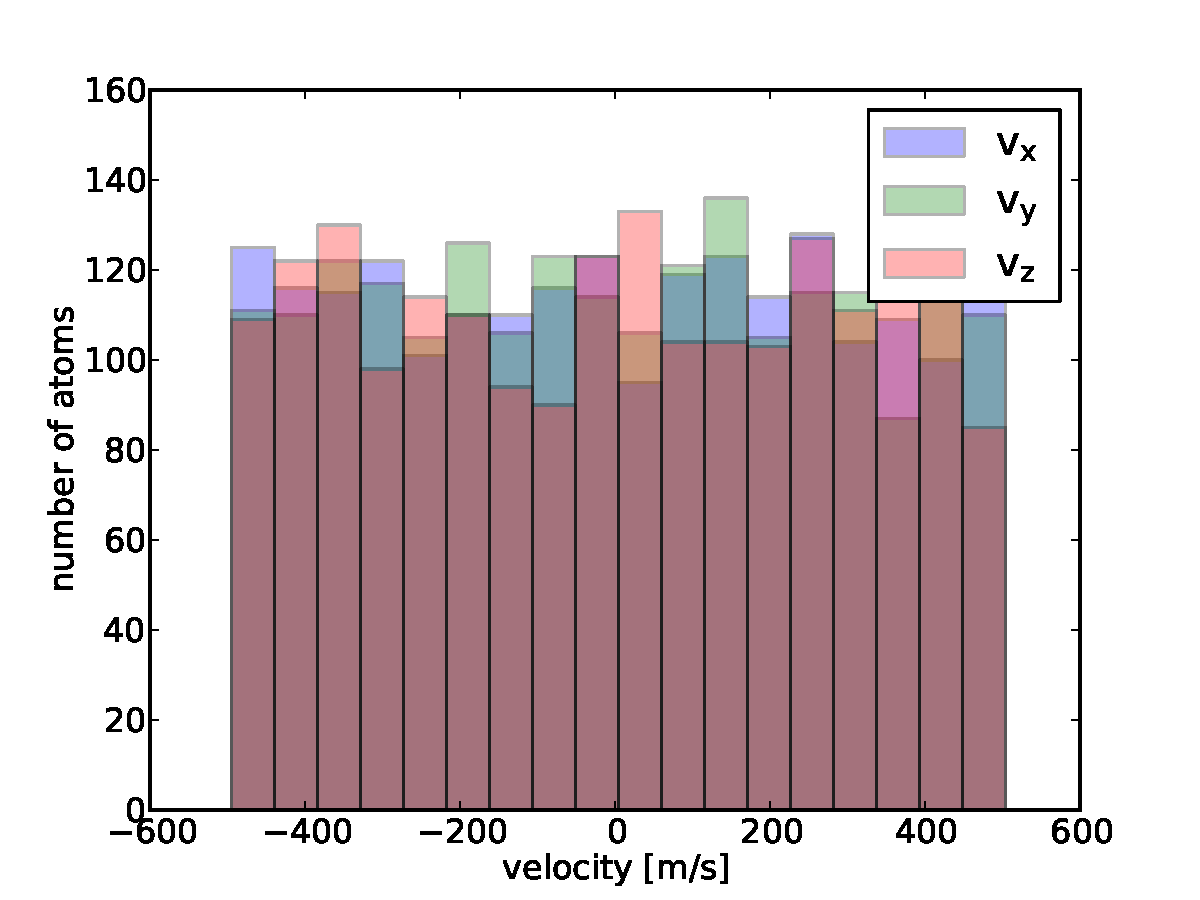
\includegraphics[width=0.48\textwidth]{./analysis/1i-boltzmann/runs/2013-02-26_180246/data000000-comp.pdf}
    } \label{fig:velocity-components-first}
    % fitness0.pdf: 576x432 pixel, 72dpi, 20.32x15.24 cm, bb=0 0 576 432
    \caption{Magnitudes (a) and components (b) of the velocities in the first time step after initializing with random uniform velocities in each direction, showing a non-Boltzmann distribution.}
    \label{fig:velocity-evolution-first}
\end{figure*}

\begin{figure*}
    \centering
    \subfigure[]{
        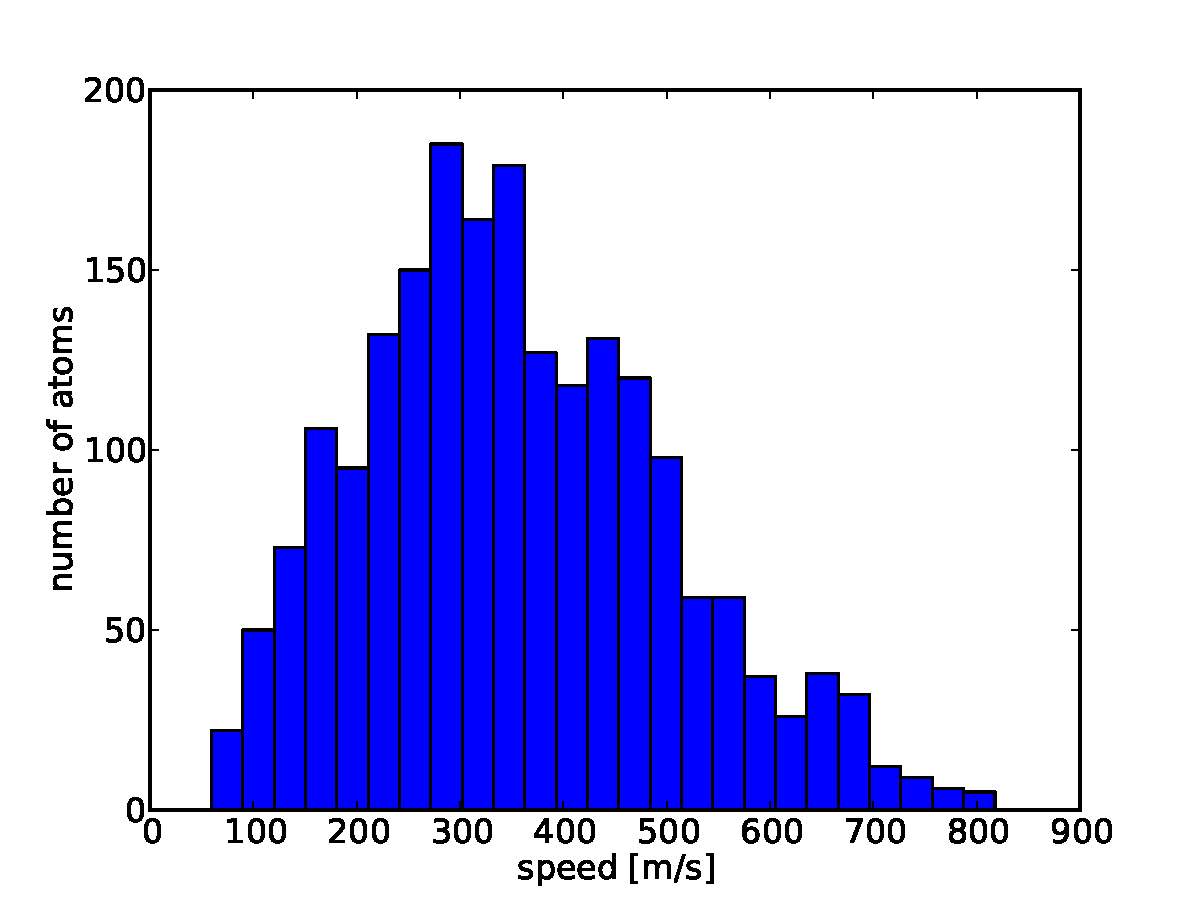
\includegraphics[width=0.48\textwidth]{./analysis/1i-boltzmann/runs/2013-02-26_180246/data000095-norm.pdf}
    } \label{fig:velocity-magnitudes-later}
    \subfigure[]{
	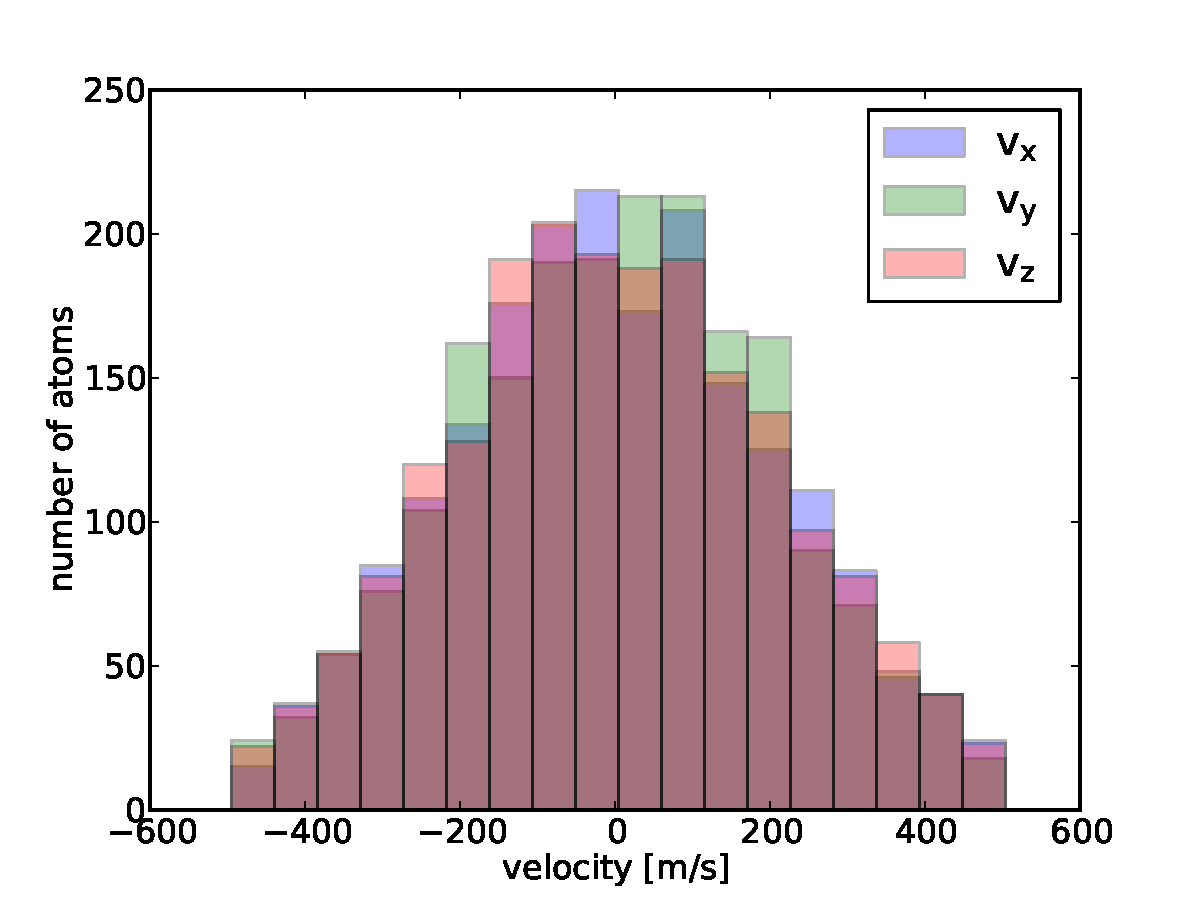
\includegraphics[width=0.48\textwidth]{./analysis/1i-boltzmann/runs/2013-02-26_180246/data000095-comp.pdf}
    } \label{fig:velocity-magnitudes-later}
    % fitness0.pdf: 576x432 pixel, 72dpi, 20.32x15.24 cm, bb=0 0 576 432
    \caption{Magnitudes (a) and components (b) of the velocities 100 time steps after initializing with random uniform velocities in each direction. This clearly shows a Boltzmann distribution of the magnitudes and a normal distribution of the components.}
    \label{fig:velocity-evolution-later}
\end{figure*}

\subsection{Energy fluctuations based on time step}

\begin{figure*}
    \centering
    \subfigure[~ $\Delta t = 1.2 \cdot 10^{-14} \unit{s}$]{
        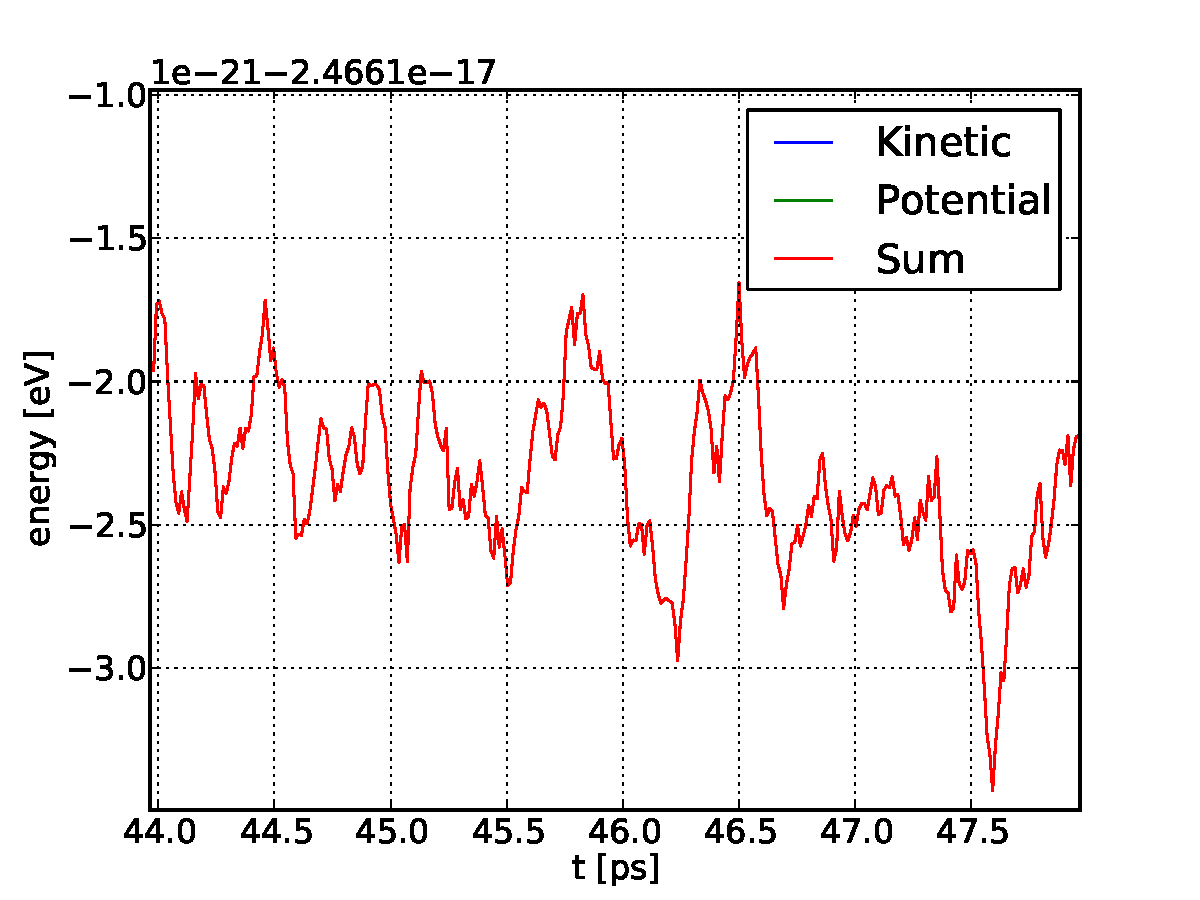
\includegraphics[width=0.48\textwidth]{./analysis/1j-energy/runs/2013-02-25_140300/energy-0001.pdf}
    } \label{fig:energy-fluctuations-small}
    \subfigure[~ $\Delta t = 5.6 \cdot 10^{-14} \unit{s}$]{
        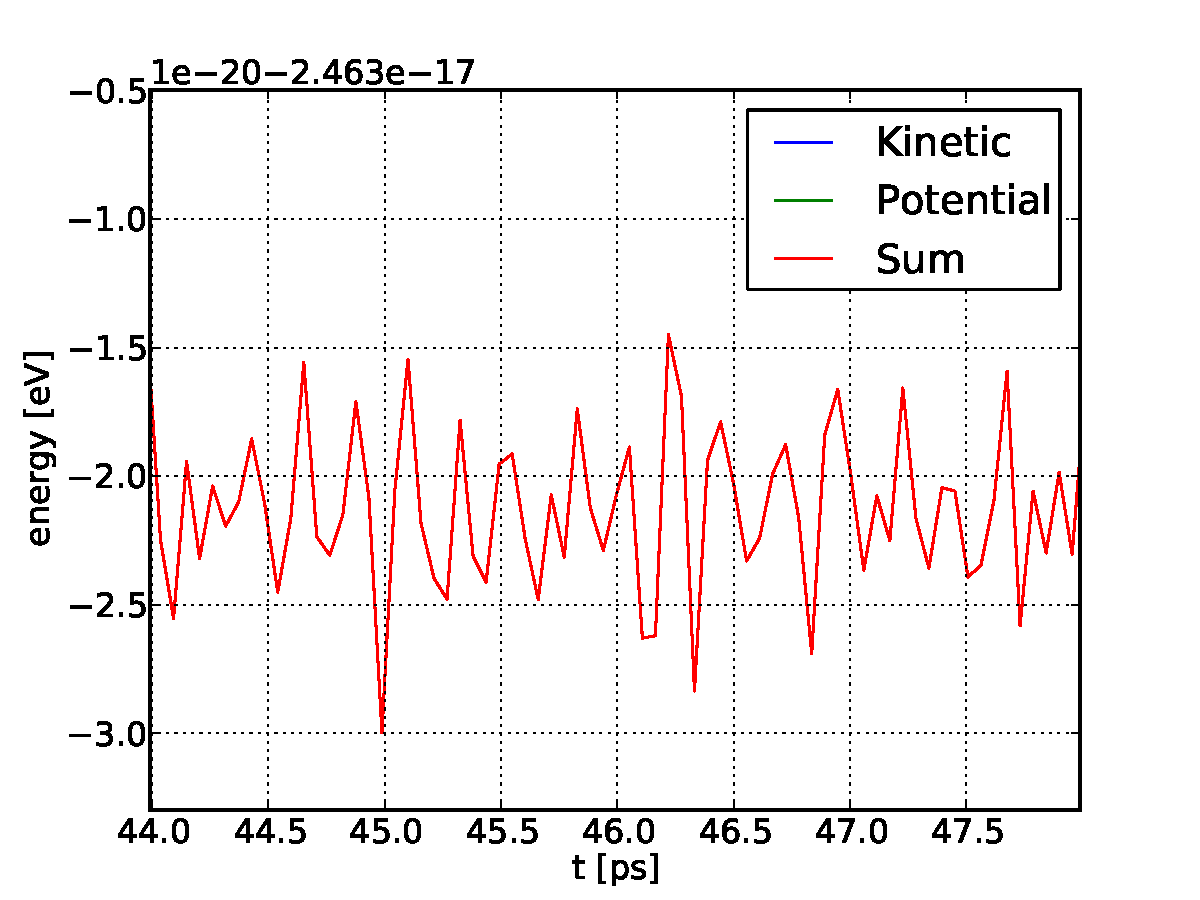
\includegraphics[width=0.48\textwidth]{./analysis/1j-energy/runs/2013-02-25_140300/energy-0005.pdf}
    } \label{fig:energy-fluctuations-large}
    % fitness0.pdf: 576x432 pixel, 72dpi, 20.32x15.24 cm, bb=0 0 576 432
    \caption{Fluctuations in kinetic energy as for a small time step (a) and a large time step (b).}
    \label{fig:energy-fluctuations}
\end{figure*}

From figure \ref{fig:energy-fluctuations} we see that the energy fluctuations do not vary much with time step, at least not in terms of frequency nor magnitude. However, figure \ref{fig:energy-fluctuations}b indicates that any larger time step than this would cause errors since the frequency of time steps would be smaller than the frequency of the fluctuations. In fact it does, and tests show that larger time steps yield non-conserved energies, as shown in figure \ref{fig:energy-fluctuations-larger}.

\begin{figure}
  \centering
  \includegraphics[width=0.48\textwidth]{./analysis/1j-energy/runs/2013-02-25_140300/energy-0006.pdf}
  \caption{Kinetic energy for a large time step $\Delta t = 6.7 \cdot 10^{-14} \unit{s}$. We clearly see that the energy diverges - a feature not shown for smaller time steps.}
  \label{fig:energy-fluctuations-larger}
\end{figure}

\subsection{Temperature evolution}

\begin{figure}
  \centering
  \includegraphics[width=0.48\textwidth]{./analysis/1k-temperature/runs/2013-02-25_182713/systemsize0009/temperature-start.pdf}
  \caption{Kinetic energy for a large time step $\Delta t = 6.7 \cdot 10^{-14} \unit{s}$. We clearly see that the energy diverges - a feature not shown for smaller time steps.}
  \label{fig:temperature-evolution}
\end{figure}

If we start the system at $T = 300 \unit{K}$ in a perfect fcc grid, we won't stay at this temperature throughout the run. The reason is that the potential energy is practically zero in an fcc grid. We see this effect in figure \ref{fig:temperature-evolution}.

\subsection{Temperature fluctuations based on system size}

\begin{figure*}
    \centering
    \subfigure[~ System size $6 \times 6 \times 6$]{
        \includegraphics[width=0.48\textwidth]{./analysis/1k-temperature/runs/2013-02-25_182713/systemsize0006/temperature-fluctuations.pdf}
    } \label{fig:temperature-fluctuations-small}
    \subfigure[~ System size $12 \times 12 \times 12$]{
        \includegraphics[width=0.48\textwidth]{./analysis/1k-temperature/runs/2013-02-25_182713/systemsize0012/temperature-fluctuations.pdf}
    } \label{fig:temperature-fluctuations-large}
    % fitness0.pdf: 576x432 pixel, 72dpi, 20.32x15.24 cm, bb=0 0 576 432
    \caption{Fluctuations in temperature for a small system (a) and a large system (b).}
    \label{fig:temperature-fluctuations}
\end{figure*}



% \begin{figure}
%  \centering
%  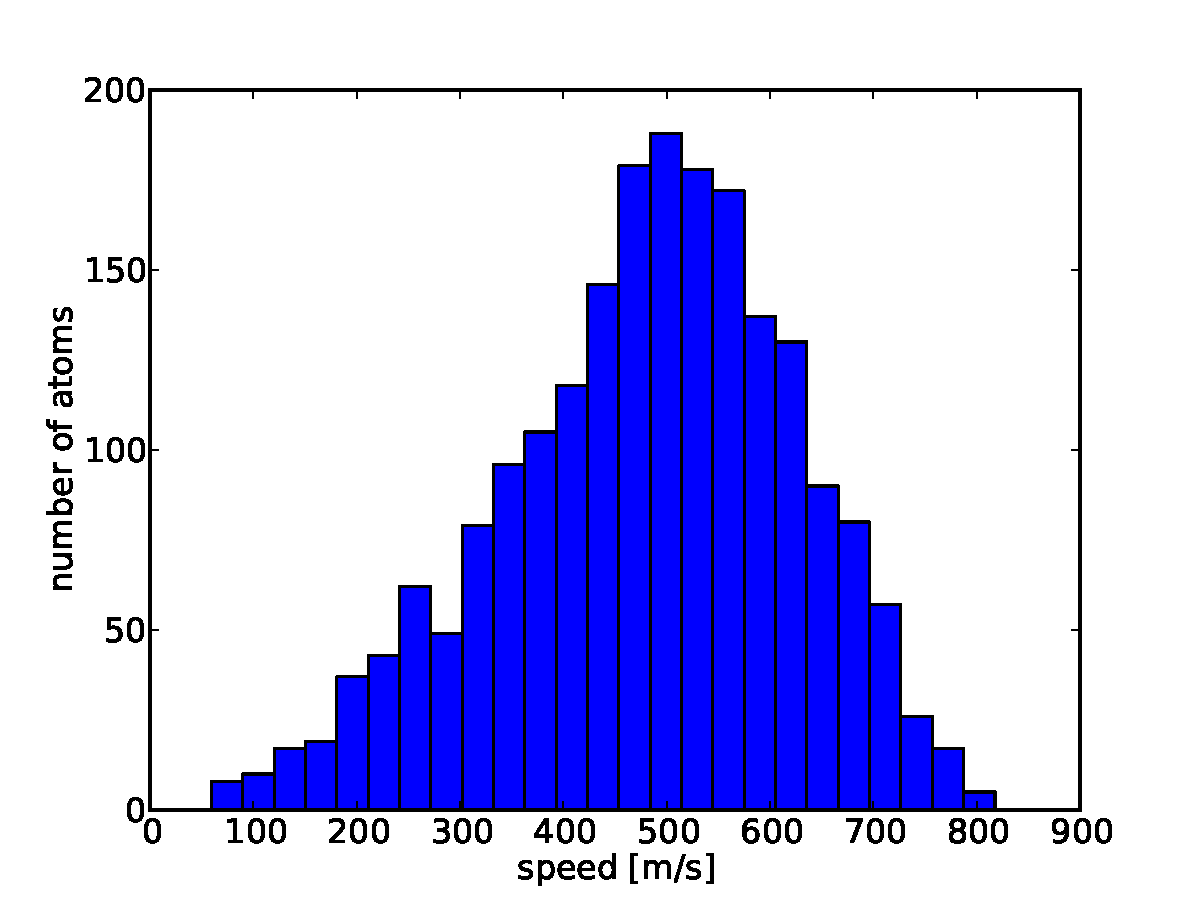
\includegraphics[width=0.5\textwidth]{./analysis/1i-boltzmann/runs/2013-02-26_180246/data000000-norm.pdf}
%  % data000000.bin-norm.pdf: 576x432 pixel, 72dpi, 20.32x15.24 cm, bb=0 0 576 432
%  \caption{Magnitudes of the velocities in the first time step after initializing with random uniform velocities in each direction, showing a non-Boltzmann distribution.}
%  \label{fig:velocity-magnitudes}
% \end{figure}
% \begin{figure}
%  \centering
%  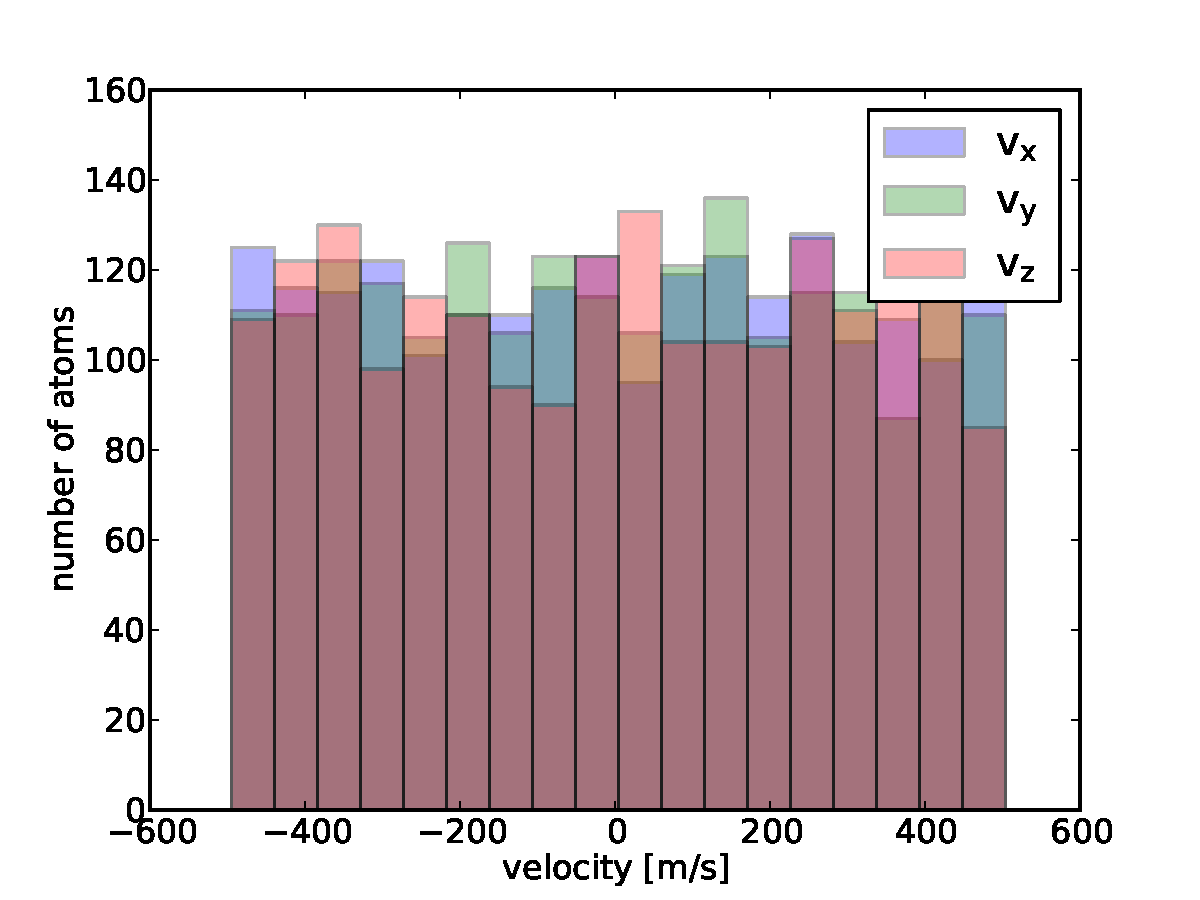
\includegraphics[width=0.5\textwidth]{./analysis/1i-boltzmann/runs/2013-02-26_180246/data000000-comp.pdf}
%  % data000000.bin-norm.pdf: 576x432 pixel, 72dpi, 20.32x15.24 cm, bb=0 0 576 432
%  \caption{Components of the velocities in the first time step after initializing with random uniform velocities in each direction, showing a non-Boltzmann distribution.}
%  \label{fig:velocity-magnitudes}
% \end{figure}



\appendix

\section{Conversion to atomic units}

\bibliographystyle{abbrvnat}
\bibliography{references}

\end{document}
